% Chapter 5 — Methodology and System Design
% For inclusion in the diploma thesis main .tex file via \input{} or \include{}
% Requires: graphicx, booktabs, longtable, hyperref packages in the preamble.
% Compile: pdflatex → bibtex → pdflatex → pdflatex  (or latexmk -pdf)

\chapter{Methodology and System Design}
\label{ch:methodology}

% ============================================================================
\section{Methodology of the Work}
\label{sec:methodology}

\subsection{Software Development Life Cycle Approach}
\label{subsec:sdlc}

The development of the Discrete Math Calculator (DMC) platform followed an iterative, incremental methodology grounded in the Agile framework, with specific practices drawn from Scrum. This approach was selected for several reasons directly relevant to the nature of the project. First, the DMC platform is a multi-tier web application integrating heterogeneous technologies---a Java backend, a Python computational engine, and a React frontend---where requirements evolve as the interplay between components becomes clearer during implementation. Second, the educational domain introduces inherent uncertainty: pedagogical features such as adaptive difficulty and AI-driven problem generation require empirical validation with real interaction patterns, making upfront waterfall-style specification impractical. Third, as a diploma project developed by a single author under academic supervision, the feedback loop between supervisor review and development iterations maps naturally onto the Scrum sprint cycle, where each sprint concludes with a demonstrable increment reviewed by a stakeholder.

The project was organized into five development phases (referred to as ``waves'' in the internal documentation), each corresponding to a thematic milestone. Wave~1 established the computational engine and basic frontend calculator. Wave~2 introduced the Spring Boot backend with authentication, database migrations, and the API gateway pattern. Wave~3 built the educational domain: courses, lessons, teacher roles, problem templates, and AI-driven problem generation with hybrid verification. Wave~4 implemented Bayesian Knowledge Tracing for adaptive difficulty selection. Wave~5 refined integration, testing, and documentation for diploma submission.

Within each wave, work was decomposed into user stories expressed in the standard format: ``As a [role], I want to [action] so that [benefit].'' Each story carried acceptance criteria specifying both functional behavior and non-functional constraints (response time under 3~seconds for computation endpoints, minimum 80\% test coverage for the math engine). A product backlog was maintained as a prioritized list of stories; at the start of each sprint (typically one to two weeks), the highest-priority stories were selected for the sprint backlog based on estimated effort and dependencies.

\subsection{Artifacts and Ceremonies}
\label{subsec:artifacts}

The primary artifacts produced during the development process include the product backlog (tracked in the repository issue tracker and internal Markdown files), sprint backlogs for each wave, the Flyway migration history (V1 through V14) serving as a versioned record of schema evolution, an architectural review document (\texttt{REVIEWS.md}) functioning as a living architecture decision record, and automated test suites (88 tests for the math engine at the time of writing). Code review was performed through pull requests, with each merge requiring a passing CI pipeline (lint checks via flake8, unit and integration tests via pytest, and compilation verification via Maven).

Sprint retrospectives after each wave produced actionable improvements. For example, after Wave~2 the retrospective identified that direct frontend-to-math-engine communication bypassed authentication, leading to the API gateway refactoring in Wave~3. After Wave~3, the retrospective noted the absence of a student knowledge model, directly motivating the BKT implementation in Wave~4.

\subsection{Risk Management}
\label{subsec:risks}

The following risks were identified at the project inception and managed throughout development.

\textbf{Technical risk: LLM reliability.} The dependence on Google Gemini for problem generation and semantic answer verification introduces a risk of hallucinated or incorrect outputs. This was mitigated by the hybrid verification architecture: SymPy provides deterministic symbolic checking as the primary verification path, with LLM verification used only when symbolic methods cannot be applied. A confidence score is returned with every LLM judgment, allowing the frontend to display appropriate caveats.

\textbf{Technical risk: Inter-service coupling.} The three-tier architecture creates inter-service dependencies where the failure of one component can cascade. This was mitigated by implementing structured error handling in the API gateway (\texttt{CalculatorProxyService} maps math engine failures to typed error codes such as \texttt{MATH\_ENGINE\_ERROR} and \texttt{MATH\_ENGINE\_UNAVAILABLE}), providing fallback problem templates when AI generation fails, and designing the frontend to degrade gracefully with informative error messages.

\textbf{Schedule risk: Scope creep.} The educational domain is vast, and the temptation to implement features such as collaborative learning, spaced repetition, and gamification simultaneously was managed through strict MoSCoW prioritization (detailed in Section~\ref{sec:mvp}). Only Must-have features were committed to the diploma scope; Should-have features were documented as future work.

\textbf{External dependency risk: API cost and rate limits.} The Gemini API has per-minute token limits and per-month cost ceilings. This was addressed by implementing a template-based generation mode as an alternative to AI generation, caching generated problems in the database (JSONB snapshots in the \texttt{generated\_problems} table), and planning Redis-based response caching for frequently requested computations.


% ============================================================================
\section{System Architecture}
\label{sec:architecture}

\subsection{Architectural Overview}
\label{subsec:arch-overview}

The DMC platform employs a three-tier client-server architecture augmented with a dedicated AI/computation microservice. The architecture separates concerns along three axes: presentation (React SPA), business logic and orchestration (Spring Boot backend), and domain computation with AI integration (FastAPI math engine). This separation allows each tier to be developed, tested, and scaled independently, and it reflects the principle that computationally intensive symbolic algebra and LLM API calls should not share resources with the authentication and data persistence layer.

In production, Nginx serves the compiled React application as static files and reverse-proxies API requests to the appropriate backend service based on URL prefix: \texttt{/api/v1/*} routes to the math engine, and \texttt{/api/*} routes to the Spring Boot backend. In development, the Vite development server handles proxying transparently.

\subsection{Frontend Architecture}
\label{subsec:frontend-arch}

The frontend is a single-page application built with React~18, bundled by Vite, and styled with Tailwind CSS~3. React Router~6 manages client-side navigation with a subject-first URL scheme. The application supports five mathematical subjects with a total of 32 interactive calculator modules: Discrete Mathematics (7), Linear Algebra (8), Algorithms and Data Structures (8), Probability and Statistics (4), and Logic and Computation (5).

Authentication state is managed through a React Context (\texttt{AuthContext}) that wraps the entire application. Protected routes are enforced by a \texttt{ProtectedRoute} component. API communication is centralized in a single \texttt{api.js} module that attaches JWT credentials to all requests.

\subsection{Backend Architecture}
\label{subsec:backend-arch}

The backend is a Spring Boot 3.2.5 application running on Java~21, structured into four bounded contexts following domain-driven design principles:

\begin{enumerate}
  \item \textbf{Authentication context} (\texttt{com.dmc.auth}): user registration, login, JWT issuance, refresh token rotation with replay detection, session management, password reset, and account lockout.
  \item \textbf{Learning context} (\texttt{com.dmc.learning}): CRUD for courses, modules, and lessons; role-restricted writes (ADMIN/TEACHER); lesson progress tracking.
  \item \textbf{Problem context} (\texttt{com.dmc.problem}): static problems, problem templates, topic taxonomy, AI-generated problems with JSONB snapshots, attempts, and BKT student skills.
  \item \textbf{Calculator gateway} (\texttt{com.dmc.problem.controller}): API gateway pattern proxying all math engine requests with \texttt{X-Internal-Api-Key} header.
\end{enumerate}

The database schema is managed by Flyway with 14 versioned migrations (V1--V14).

\subsection{Math Engine Architecture}
\label{subsec:math-engine-arch}

The math engine is a FastAPI application running on Uvicorn, exposing 12 domain-specific calculator routers plus specialized routers for problem generation, verification, AI chat, and OCR. The computational core uses SymPy for symbolic algebra, NumPy for numerical operations, and NetworkX for graph algorithms. The AI module (\texttt{dmc\_ai}) integrates Google Gemini as the primary LLM with Groq as a fallback.

The hybrid verification system attempts symbolic verification via SymPy first (\texttt{simplify(expected - student) == 0}), falls back to semantic verification via Gemini (returning correctness, confidence, and feedback), and uses string comparison as a last resort.

\subsection{Inter-Service Communication}
\label{subsec:inter-service}

All inter-service communication uses synchronous HTTP/JSON. The backend communicates with the math engine via Java's \texttt{HttpClient}, with configurable timeouts. Inter-service authentication uses a shared secret key (\texttt{X-Internal-Api-Key} header). The infrastructure layer includes PostgreSQL~16, Redis~7 (deployed; integration planned), and RabbitMQ~3.13 (deployed; async tasks planned).


% ============================================================================
\section{UML Diagrams}
\label{sec:uml}

This section presents five UML diagrams modeling the DMC platform's structure and behavior. Source files in PlantUML format are available in the \texttt{diagrams/} directory.

\subsection{Use Case Diagram}
\label{subsec:use-case}

% \begin{figure}[htbp]
%   \centering
%   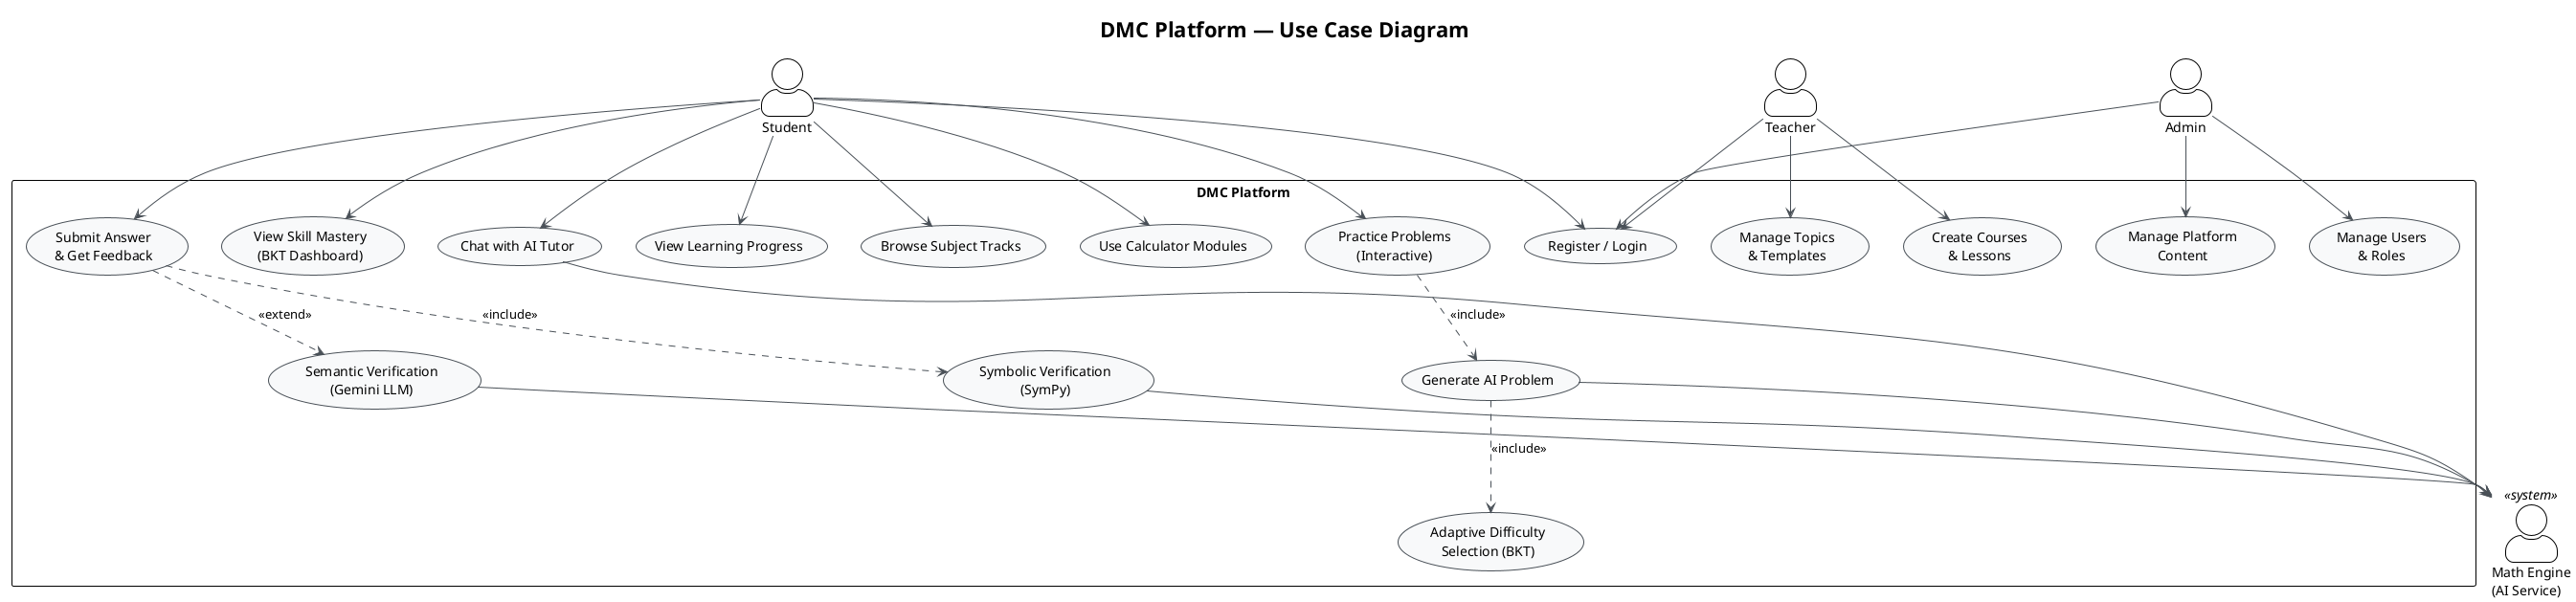
\includegraphics[width=\textwidth]{figures/use_case_diagram.png}
%   \caption{Use Case Diagram of the DMC Platform}
%   \label{fig:use-case}
% \end{figure}

The Use Case diagram (Figure~\ref{fig:use-case}) identifies three primary actors---Student, Teacher, and Admin---and one system actor (Math Engine). The Student interacts through eight use cases spanning the complete learning lifecycle. The Teacher manages topics, templates, courses, and lessons. The Admin manages users and platform content. Critical relationships include: Interactive Practice \textit{includes} Generate AI Problem, which in turn \textit{includes} Adaptive Difficulty Selection via BKT; Submit Answer \textit{includes} Symbolic Verification and \textit{extends} to Semantic Verification.

\subsection{Sequence Diagram --- Solve a Generated Problem}
\label{subsec:sequence}

% \begin{figure}[htbp]
%   \centering
%   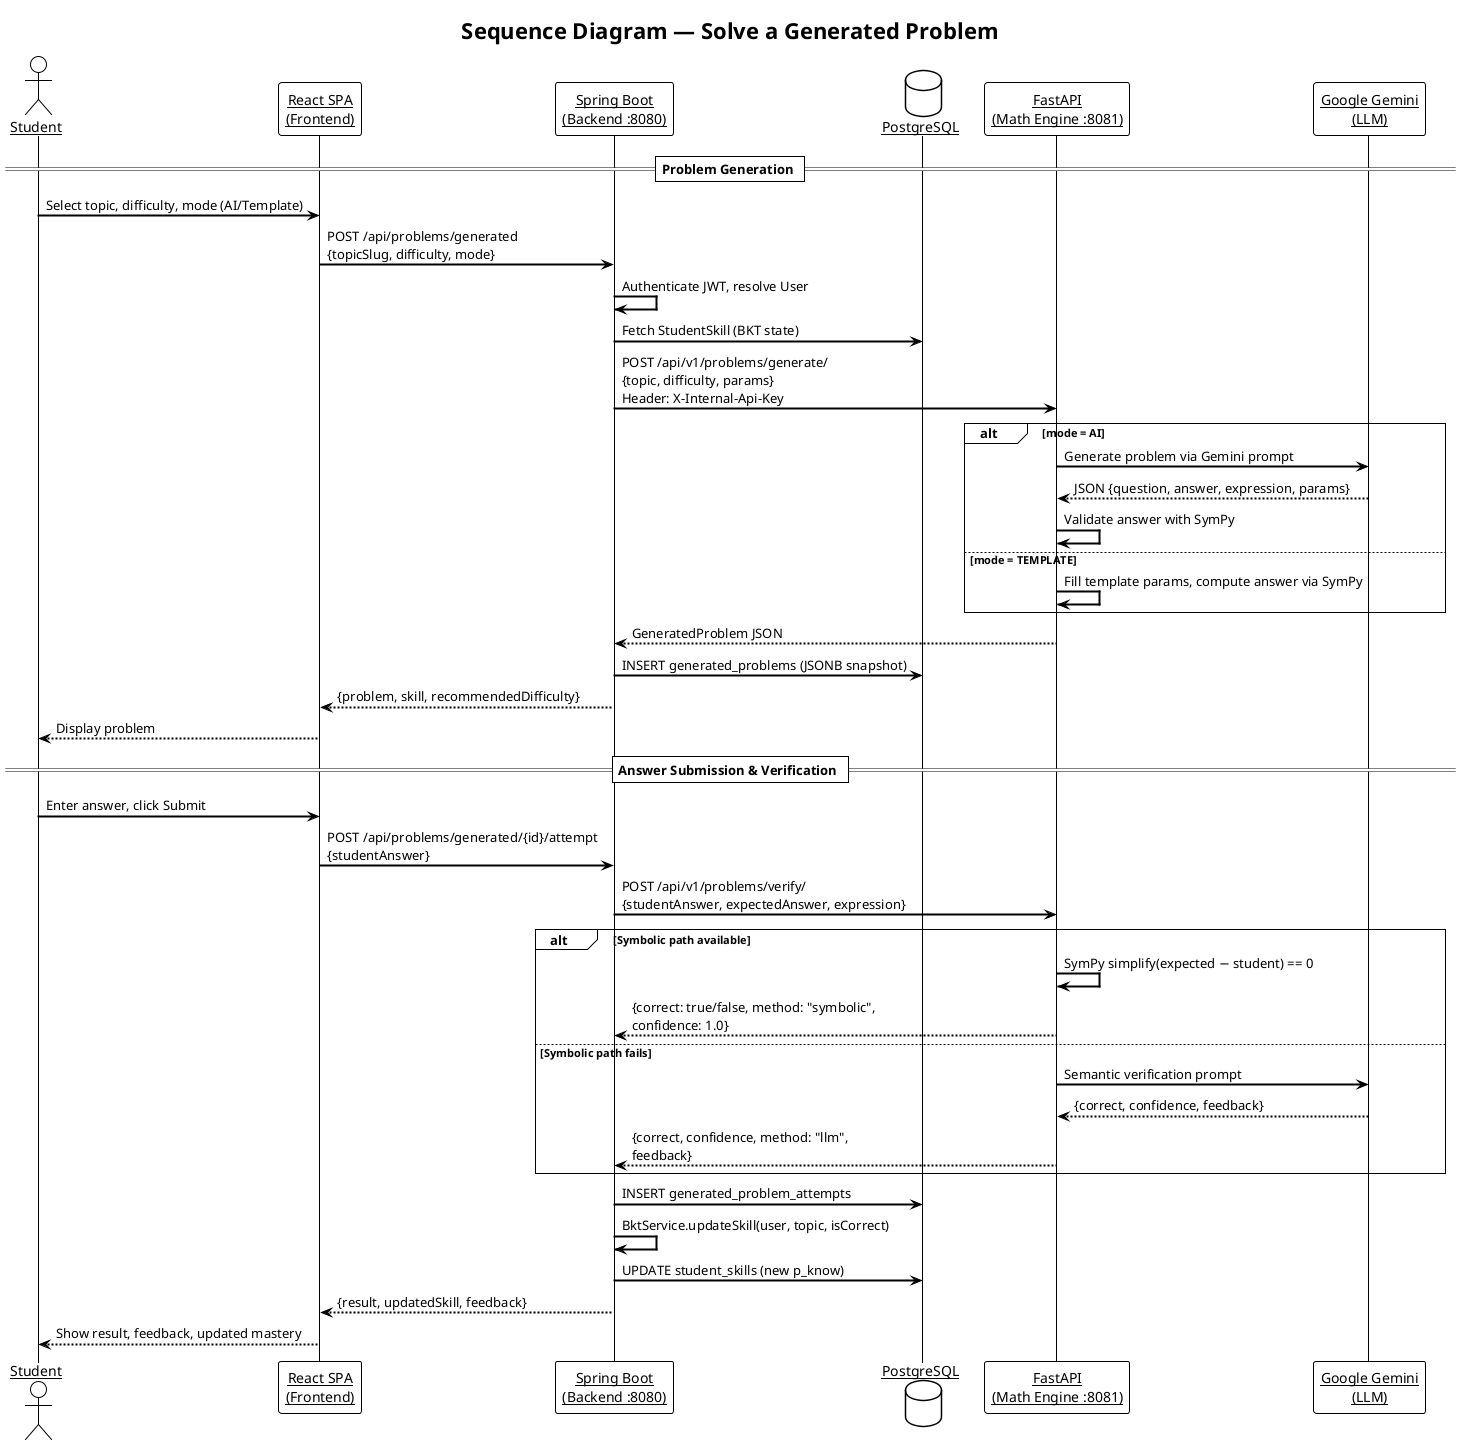
\includegraphics[width=\textwidth]{figures/sequence_solve_problem.png}
%   \caption{Sequence Diagram: Solving a Generated Problem}
%   \label{fig:sequence}
% \end{figure}

The Sequence diagram (Figure~\ref{fig:sequence}) traces the complete interaction for the core educational scenario. Five lifelines participate: Student, React SPA, Spring Boot backend, PostgreSQL, and FastAPI math engine. The flow divides into Generation (topic selection $\rightarrow$ BKT state fetch $\rightarrow$ problem generation via AI or Template $\rightarrow$ JSONB persistence) and Verification (answer submission $\rightarrow$ symbolic/semantic verification $\rightarrow$ BKT update $\rightarrow$ feedback display).

\subsection{Activity Diagram --- Adaptive Learning Flow}
\label{subsec:activity}

% \begin{figure}[htbp]
%   \centering
%   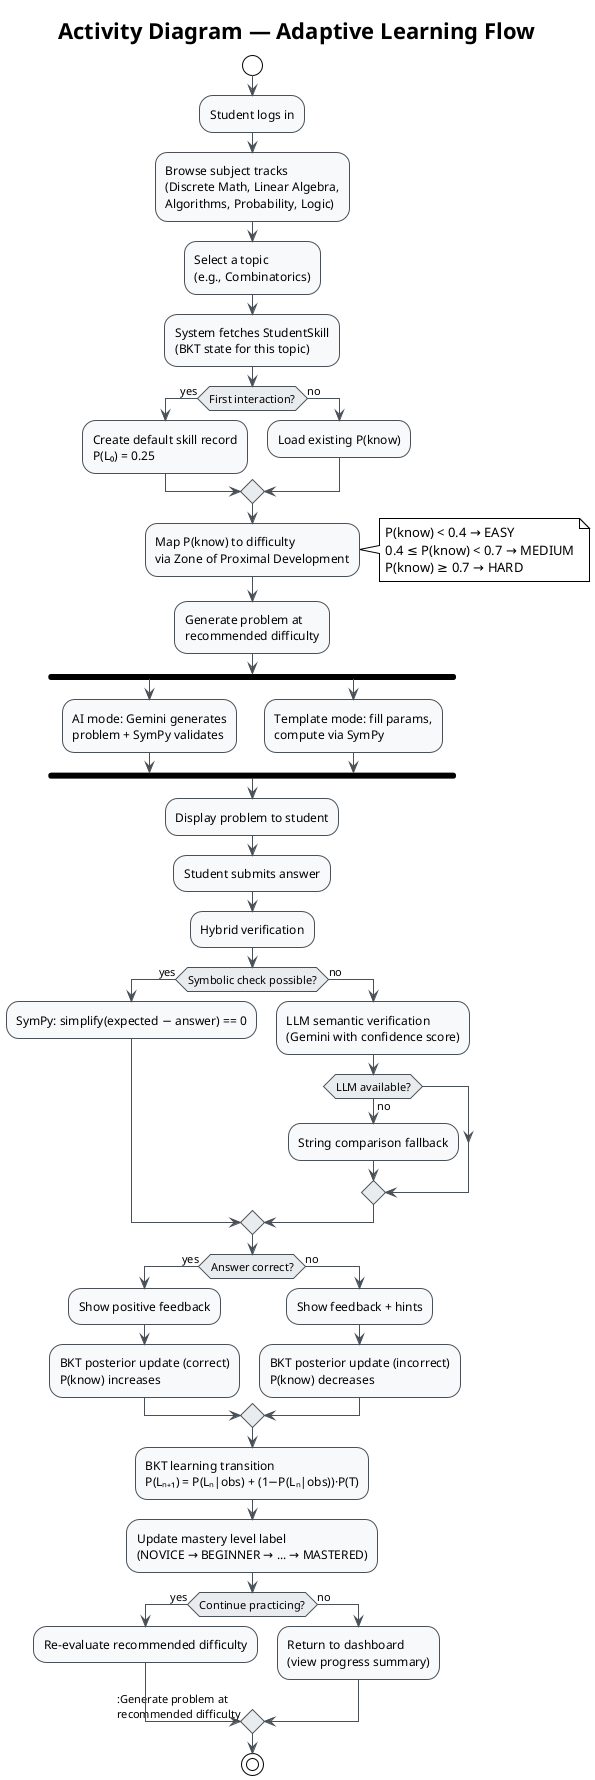
\includegraphics[width=\textwidth]{figures/activity_learning_flow.png}
%   \caption{Activity Diagram: Adaptive Learning Flow}
%   \label{fig:activity}
% \end{figure}

The Activity diagram (Figure~\ref{fig:activity}) models the adaptive learning loop: authentication $\rightarrow$ subject/topic selection $\rightarrow$ BKT difficulty mapping (P(know) thresholds to Easy/Medium/Hard via Zone of Proximal Development) $\rightarrow$ problem generation (AI or Template fork) $\rightarrow$ hybrid verification (symbolic $\rightarrow$ LLM $\rightarrow$ fallback) $\rightarrow$ BKT posterior update $\rightarrow$ loop.

\subsection{Component Diagram}
\label{subsec:component}

% \begin{figure}[htbp]
%   \centering
%   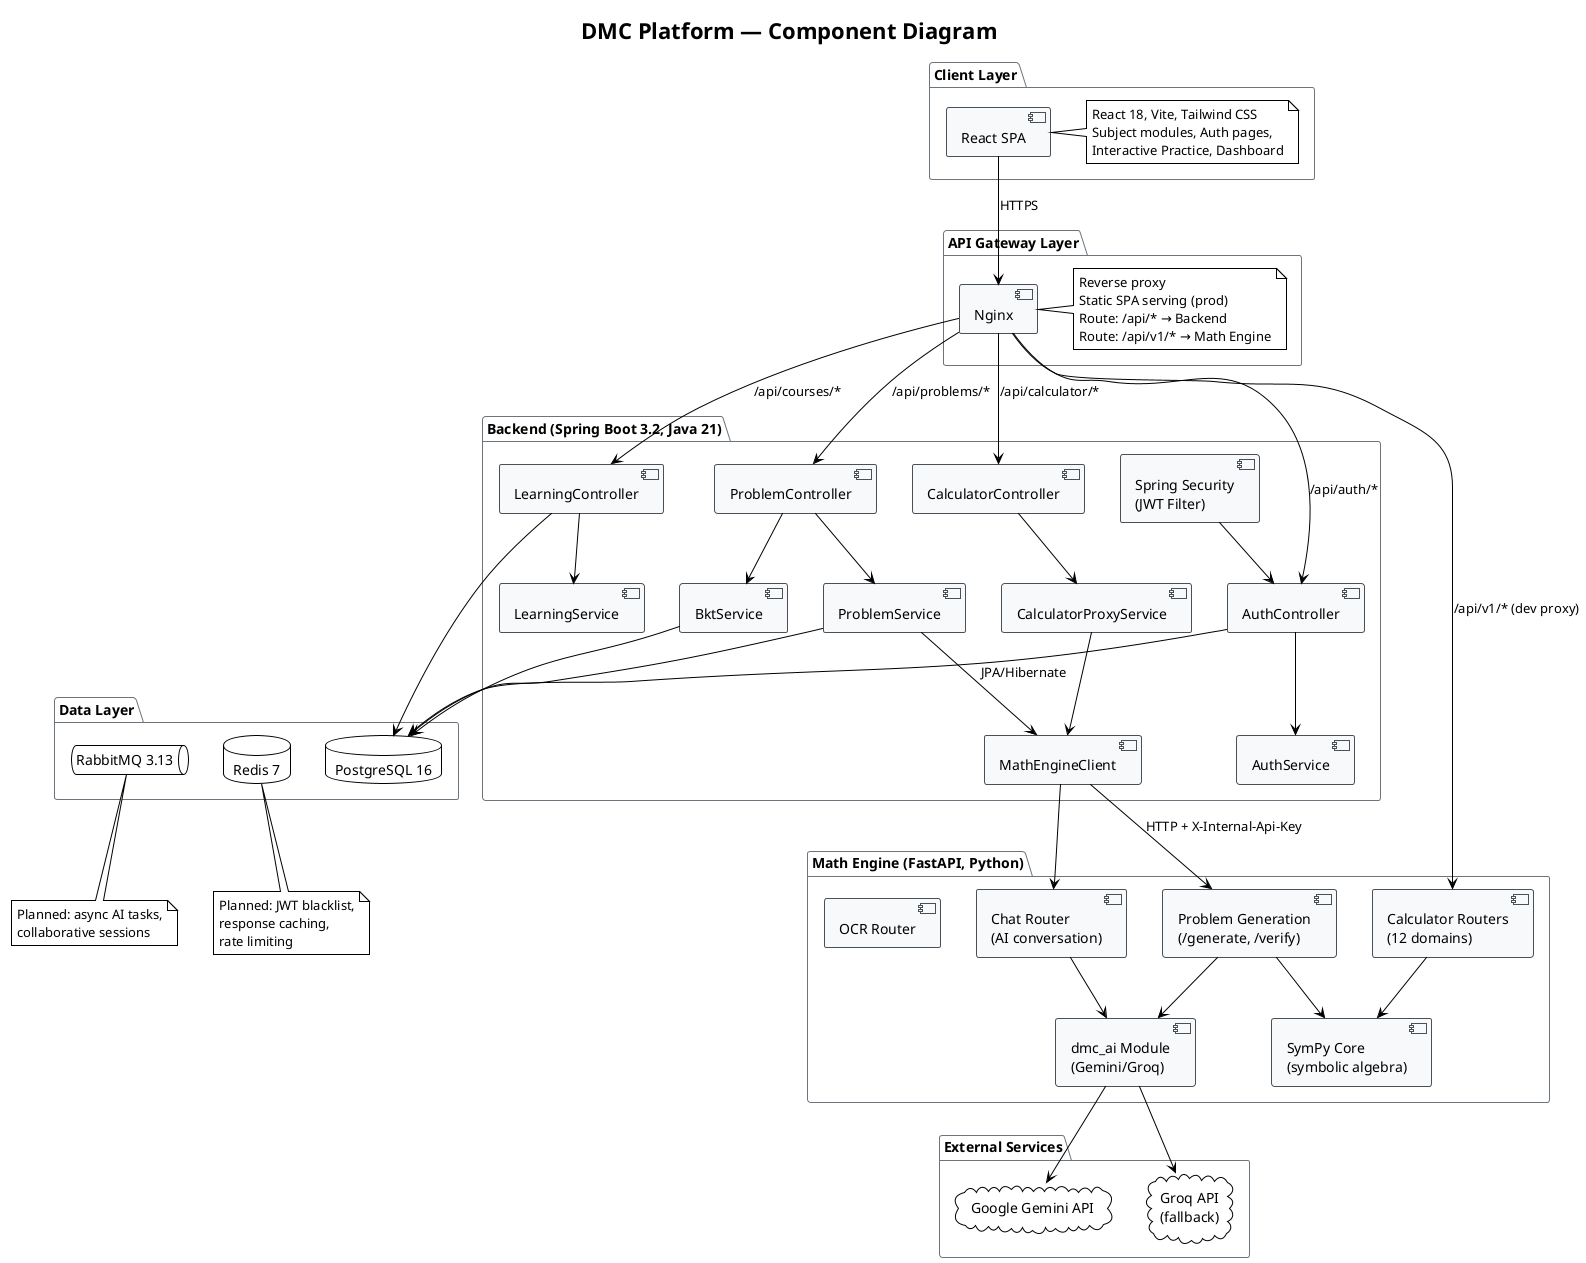
\includegraphics[width=\textwidth]{figures/component_diagram.png}
%   \caption{Component Diagram of the DMC Platform}
%   \label{fig:component}
% \end{figure}

The Component diagram (Figure~\ref{fig:component}) decomposes the system into five packages: Client Layer, API Gateway Layer, Backend (controllers, services, MathEngineClient), Math Engine (routers, SymPy core, dmc\_ai), and Data Layer (PostgreSQL, Redis, RabbitMQ).

\subsection{Deployment Diagram}
\label{subsec:deployment}

% \begin{figure}[htbp]
%   \centering
%   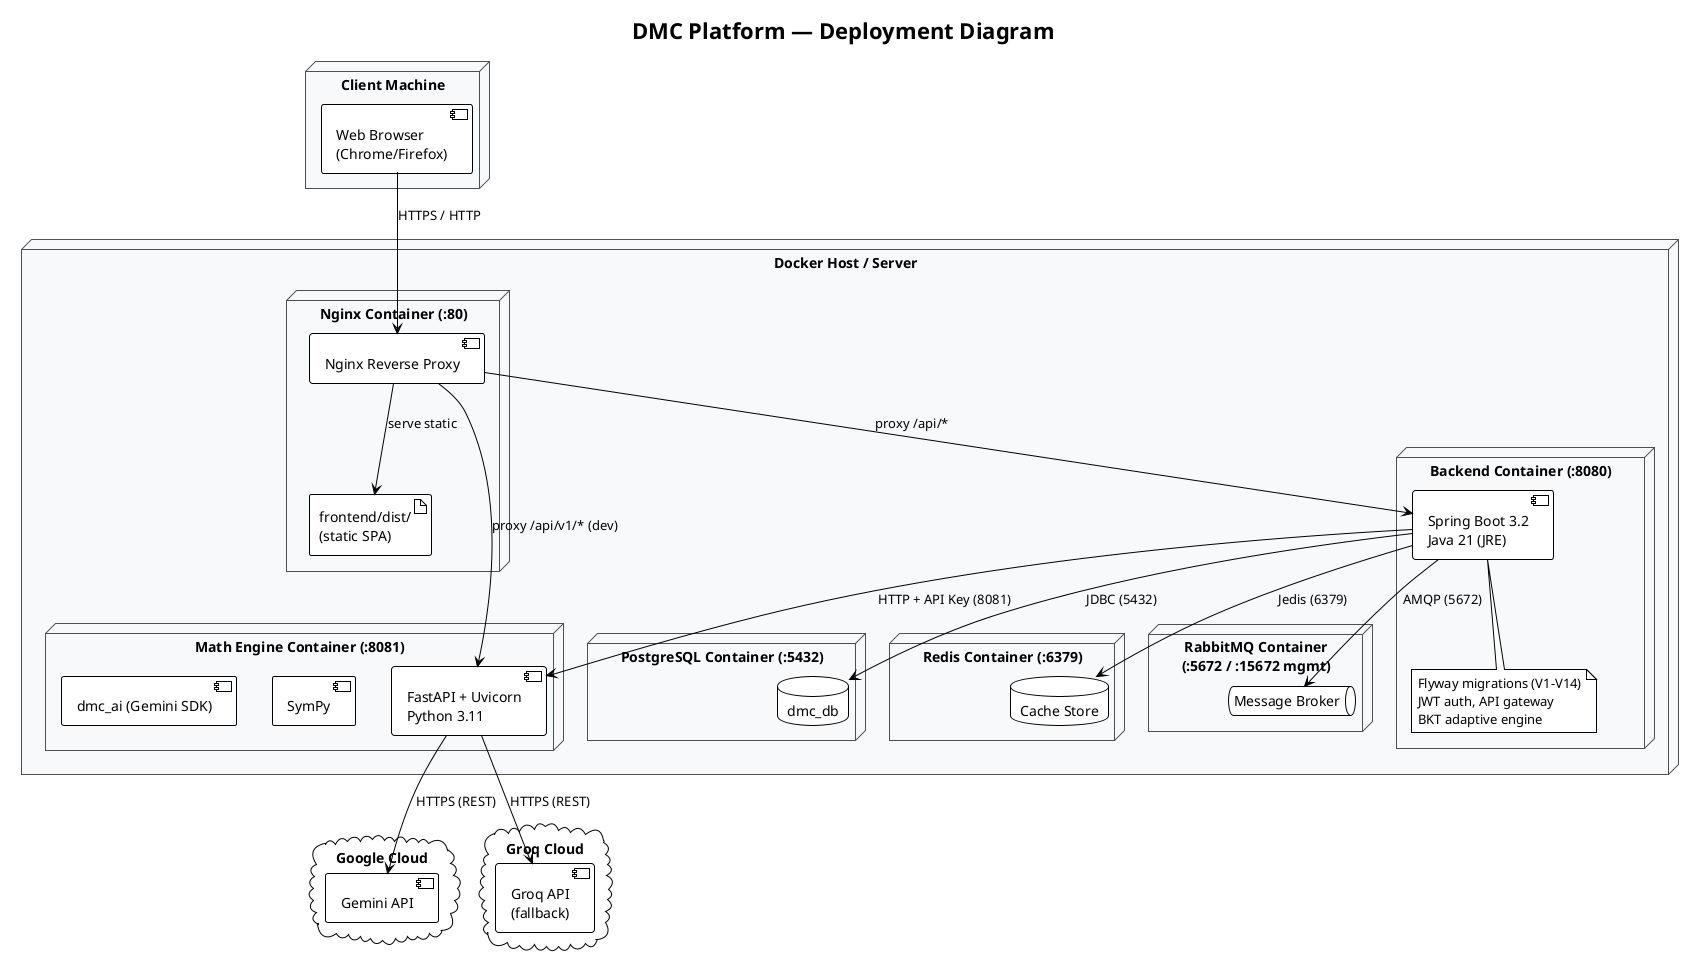
\includegraphics[width=\textwidth]{figures/deployment_diagram.png}
%   \caption{Deployment Diagram of the DMC Platform}
%   \label{fig:deployment}
% \end{figure}

The Deployment diagram (Figure~\ref{fig:deployment}) maps components to Docker containers: Nginx (:80), Spring Boot (:8080), FastAPI (:8081), PostgreSQL (:5432), Redis (:6379), and RabbitMQ (:5672/15672). External cloud dependencies (Gemini API, Groq API) are shown as separate nodes. Production hardening includes \texttt{no-new-privileges}, \texttt{cap\_drop: ALL}, read-only filesystems, resource limits, and non-root users.


% ============================================================================
\section{MVP Scope}
\label{sec:mvp}

\subsection{MoSCoW Prioritization}
\label{subsec:moscow}

The MVP scope was defined using MoSCoW prioritization, balancing the academic requirements of the diploma topic with practical constraints.

\textbf{Must-have} (implemented):
\begin{itemize}
  \item Multi-subject calculator with 32 modules across 5 subjects
  \item JWT authentication with refresh token rotation and account lockout
  \item Role-based access: Student, Teacher, Admin
  \item Course/lesson management (CRUD) for Teachers/Admins
  \item Topic taxonomy with normalized slugs
  \item Problem templates and AI-driven problem generation
  \item Hybrid verification: symbolic (SymPy) $\rightarrow$ semantic (Gemini) $\rightarrow$ string fallback
  \item BKT adaptive difficulty with ZPD mapping
  \item API gateway with inter-service authentication
  \item AI chatbot, calculation history, 88 math engine tests, 14 Flyway migrations
\end{itemize}

\textbf{Should-have} (documented as future work): learning analytics dashboard, progressive hint scaffolding, Redis JWT blacklisting, caching, rate limiting, CSRF, E2E tests.

\textbf{Could-have}: spaced repetition (SM-2), error pattern analysis, collaborative sessions, gamification.

\textbf{Won't-have}: payments, mobile apps, Kubernetes, i18n.

\subsection{User Stories}
\label{subsec:user-stories}

Eleven user stories were implemented (US-01 through US-11), covering student authentication, subject browsing, calculator usage, adaptive practice, AI problem generation, hybrid verification, mastery tracking, AI chat, teacher template management, topic management, and admin user management.

\subsection{Development Roadmap}
\label{subsec:roadmap}

\begin{table}[htbp]
\centering
\caption{Development Roadmap by Wave}
\label{tab:roadmap}
\begin{tabular}{clp{8cm}}
\toprule
\textbf{Wave} & \textbf{Theme} & \textbf{Key Deliverables} \\
\midrule
1 & Computational Engine & FastAPI with 12 routers, SymPy, 88 tests, React with 32 modules \\
2 & Backend Foundation & Spring Boot, JWT auth, Flyway V1--V11, Docker, Nginx \\
3 & Educational Domain & Courses, TEACHER role, topics, templates, AI generation, hybrid verification, gateway (V12--V13) \\
4 & Adaptive Intelligence & BKT, student\_skills (V14), adaptive difficulty, mastery levels \\
5 & Integration \& Defense & Testing, documentation, architecture review, diploma chapters \\
\bottomrule
\end{tabular}
\end{table}


% ============================================================================
\section{Technology Comparison}
\label{sec:tech-comparison}

\subsection{Frontend Framework Comparison}
\label{subsec:frontend-comparison}

\begin{table}[htbp]
\centering
\caption{Frontend Framework Comparison}
\label{tab:frontend-comparison}
\begin{tabular}{p{2.5cm}p{3.5cm}p{3.5cm}p{3.5cm}}
\toprule
\textbf{Criterion} & \textbf{React 18} & \textbf{Vue 3} & \textbf{Angular 17} \\
\midrule
Performance & Virtual DOM, concurrent features & Proxy reactivity & Zone.js, Ivy compiler \\
Dev speed & High (JSX, hooks) & High (SFC, Composition API) & Moderate (boilerplate) \\
Learning curve & Moderate & Low & High \\
Community & Largest (~23M/wk npm) & Growing (~4M/wk) & Stable (~3M/wk) \\
AI/Education & Excellent (KaTeX, Recharts) & Good & Good \\
Scalability & Component-based, lazy loading & Similar & Module system \\
\bottomrule
\end{tabular}
\end{table}

React~18 was selected for its dominant ecosystem, the author's experience, Vite's fast HMR, and market relevance for AITU graduates.

\subsection{Backend Framework Comparison}
\label{subsec:backend-comparison}

\begin{table}[htbp]
\centering
\caption{Backend Framework Comparison}
\label{tab:backend-comparison}
\begin{tabular}{p{2.5cm}p{3.5cm}p{3.5cm}p{3.5cm}}
\toprule
\textbf{Criterion} & \textbf{Spring Boot 3} & \textbf{Django 5} & \textbf{Express.js} \\
\midrule
Performance & High (JVM, virtual threads) & Moderate (GIL) & Moderate (event loop) \\
Dev speed & Moderate & High (batteries) & High \\
Learning curve & High & Moderate & Low \\
Security & Excellent (Spring Security) & Good & Basic (manual) \\
DB integration & Excellent (JPA/Flyway) & Excellent (ORM) & Moderate \\
AI integration & Indirect (HTTP to Python) & Direct (Python) & Indirect \\
\bottomrule
\end{tabular}
\end{table}

Spring Boot~3 was selected to demonstrate enterprise-grade practices; the Python math engine provides direct AI/SymPy access.

\subsection{Database Comparison}
\label{subsec:db-comparison}

\begin{table}[htbp]
\centering
\caption{Database Comparison}
\label{tab:db-comparison}
\begin{tabular}{p{2.8cm}p{3.5cm}p{3.5cm}p{3cm}}
\toprule
\textbf{Criterion} & \textbf{PostgreSQL 16} & \textbf{MongoDB 7} & \textbf{MySQL 8} \\
\midrule
ACID compliance & Full & Eventual (default) & Full (InnoDB) \\
JSON support & JSONB + GIN indexes & Native BSON & JSON (limited) \\
Analytics & Window, CTE, LATERAL & Aggregation pipeline & Window, CTE \\
Migrations & Flyway, Liquibase & Schema-less & Flyway \\
Education fit & Excellent & Good & Good \\
\bottomrule
\end{tabular}
\end{table}

PostgreSQL~16 was selected for ACID integrity, JSONB (generated problem snapshots), and analytical query capabilities.

\subsection{LLM Provider Comparison}
\label{subsec:llm-comparison}

\begin{table}[htbp]
\centering
\caption{LLM Provider Comparison}
\label{tab:llm-comparison}
\begin{tabular}{p{2.5cm}p{3.5cm}p{3.5cm}p{3.5cm}}
\toprule
\textbf{Criterion} & \textbf{Google Gemini} & \textbf{OpenAI GPT-4} & \textbf{Groq (Llama 3.3)} \\
\midrule
Cost & Generous free tier & Higher, no free GPT-4 & Free tier, rate-limited \\
Math reasoning & Strong (Flash) & Excellent & Good \\
Latency & Low (Flash) & Moderate & Very low \\
Structured output & JSON schema & Function calling & JSON mode \\
\bottomrule
\end{tabular}
\end{table}

Google Gemini was selected as the primary provider; Groq serves as a fallback for high availability.


% ============================================================================
\section{Project Mockups}
\label{sec:mockups}

This section describes the six principal UI screens. Mockups were designed in Figma and exported as PNG for inclusion.

% \begin{figure}[htbp]
%   \centering
%   \includegraphics[width=0.9\textwidth]{mockups/hub.png}
%   \caption{Hub / Landing Page (developed by the author)}
%   \label{fig:mockup-hub}
% \end{figure}

\subsection{Hub / Landing Page} The entry point presents five subject tracks as cards with name, description, module count, and calculator/roadmap links.

\subsection{Sign In / Sign Up Pages} Centered card layout with inline validation, server-error display, and cross-links.

\subsection{Student Dashboard} Displays username, XP, streak, plan, and subject progress cards with a ``Practice'' entry point.

\subsection{Interactive Practice Page} Three-section layout: controls (topic, difficulty, mode), problem display with verification result, and skill state with history.

\subsection{Subject Calculator Page} Module grid leading to domain-specific calculators with step-by-step results and floating AI chatbot.

\subsection{Content Administration Page} TEACHER/ADMIN interface for topics, templates, courses, lessons, and user management.

% For each mockup, uncomment and adjust the figure environment above.
% Caption format: "Screen Name (developed by the author)"


% ============================================================================
\section{Chapter Summary}
\label{sec:ch5-summary}

This chapter has presented the complete methodological and design foundation of the DMC platform. The development followed an Agile/Scrum-inspired iterative approach organized into five waves. The system architecture employs a three-tier polyglot design: React for presentation, Spring Boot for orchestration and security, and FastAPI with SymPy for computation and AI.

Five UML diagrams formally model the system: Use Case (actor interactions), Sequence (problem-solve flow), Activity (adaptive learning loop), Component (software modules), and Deployment (Docker containers). The MVP scope was defined via MoSCoW prioritization with 14 Must-have features. Technology selections were justified through systematic comparison tables. Mockup descriptions document the six principal UI screens.

The next chapter presents the implementation details of the platform's core AI features: the hybrid verification system and the Bayesian Knowledge Tracing engine.
